\documentclass[a4paper,12pt,twoside]{memoir}

% Castellano
\usepackage[spanish,es-tabla]{babel}
\selectlanguage{spanish}
\usepackage[utf8]{inputenc}
\usepackage[T1]{fontenc}
\usepackage{lmodern} % scalable font
\usepackage{microtype}
\usepackage{placeins}

\RequirePackage{booktabs}
\RequirePackage[table]{xcolor}
\RequirePackage{xtab}
\RequirePackage{multirow}

% Links
\PassOptionsToPackage{hyphens}{url}\usepackage[colorlinks]{hyperref}
\hypersetup{
	allcolors = {red}
}

% Ecuaciones
\usepackage{amsmath}

% Rutas de fichero / paquete
\newcommand{\ruta}[1]{{\sffamily #1}}

% Párrafos
\nonzeroparskip

% Huérfanas y viudas
\widowpenalty100000
\clubpenalty100000

% Evitar solapes en el header
\nouppercaseheads

% Imagenes
\usepackage{graphicx}
\newcommand{\imagen}[2]{
	\begin{figure}[!h]
		\centering
		\includegraphics[width=0.9\textwidth]{#1}
		\caption{#2}\label{fig:#1}
	\end{figure}
	\FloatBarrier
}

\newcommand{\imagenflotante}[2]{
	\begin{figure}%[!h]
		\centering
		\includegraphics[width=0.9\textwidth]{#1}
		\caption{#2}\label{fig:#1}
	\end{figure}
}



% El comando \figura nos permite insertar figuras comodamente, y utilizando
% siempre el mismo formato. Los parametros son:
% 1 -> Porcentaje del ancho de página que ocupará la figura (de 0 a 1)
% 2 --> Fichero de la imagen
% 3 --> Texto a pie de imagen
% 4 --> Etiqueta (label) para referencias
% 5 --> Opciones que queramos pasarle al \includegraphics
% 6 --> Opciones de posicionamiento a pasarle a \begin{figure}
\newcommand{\figuraConPosicion}[6]{%
  \setlength{\anchoFloat}{#1\textwidth}%
  \addtolength{\anchoFloat}{-4\fboxsep}%
  \setlength{\anchoFigura}{\anchoFloat}%
  \begin{figure}[#6]
    \begin{center}%
      \Ovalbox{%
        \begin{minipage}{\anchoFloat}%
          \begin{center}%
            \includegraphics[width=\anchoFigura,#5]{#2}%
            \caption{#3}%
            \label{#4}%
          \end{center}%
        \end{minipage}
      }%
    \end{center}%
  \end{figure}%
}

%
% Comando para incluir imágenes en formato apaisado (sin marco).
\newcommand{\figuraApaisadaSinMarco}[5]{%
  \begin{figure}%
    \begin{center}%
    \includegraphics[angle=90,height=#1\textheight,#5]{#2}%
    \caption{#3}%
    \label{#4}%
    \end{center}%
  \end{figure}%
}
% Para las tablas
\newcommand{\otoprule}{\midrule [\heavyrulewidth]}
%
% Nuevo comando para tablas pequeñas (menos de una página).
\newcommand{\tablaSmall}[5]{%
 \begin{table}
  \begin{center}
   \rowcolors {2}{gray!35}{}
   \begin{tabular}{#2}
    \toprule
    #4
    \otoprule
    #5
    \bottomrule
   \end{tabular}
   \caption{#1}
   \label{tabla:#3}
  \end{center}
 \end{table}
}

%
%Para el float H de tablaSmallSinColores
\usepackage{float}

%
% Nuevo comando para tablas pequeñas (menos de una página).
\newcommand{\tablaSmallSinColores}[5]{%
 \begin{table}[H]
  \begin{center}
   \begin{tabular}{#2}
    \toprule
    #4
    \otoprule
    #5
    \bottomrule
   \end{tabular}
   \caption{#1}
   \label{tabla:#3}
  \end{center}
 \end{table}
}

\newcommand{\tablaApaisadaSmall}[5]{%
\begin{landscape}
  \begin{table}
   \begin{center}
    \rowcolors {2}{gray!35}{}
    \begin{tabular}{#2}
     \toprule
     #4
     \otoprule
     #5
     \bottomrule
    \end{tabular}
    \caption{#1}
    \label{tabla:#3}
   \end{center}
  \end{table}
\end{landscape}
}

%
% Nuevo comando para tablas grandes con cabecera y filas alternas coloreadas en gris.
\newcommand{\tabla}[6]{%
  \begin{center}
    \tablefirsthead{
      \toprule
      #5
      \otoprule
    }
    \tablehead{
      \multicolumn{#3}{l}{\small\sl continúa desde la página anterior}\\
      \toprule
      #5
      \otoprule
    }
    \tabletail{
      \hline
      \multicolumn{#3}{r}{\small\sl continúa en la página siguiente}\\
    }
    \tablelasttail{
      \hline
    }
    \bottomcaption{#1}
    \rowcolors {2}{gray!35}{}
    \begin{xtabular}{#2}
      #6
      \bottomrule
    \end{xtabular}
    \label{tabla:#4}
  \end{center}
}

%
% Nuevo comando para tablas grandes con cabecera.
\newcommand{\tablaSinColores}[6]{%
  \begin{center}
    \tablefirsthead{
      \toprule
      #5
      \otoprule
    }
    \tablehead{
      \multicolumn{#3}{l}{\small\sl continúa desde la página anterior}\\
      \toprule
      #5
      \otoprule
    }
    \tabletail{
      \hline
      \multicolumn{#3}{r}{\small\sl continúa en la página siguiente}\\
    }
    \tablelasttail{
      \hline
    }
    \bottomcaption{#1}
    \begin{xtabular}{#2}
      #6
      \bottomrule
    \end{xtabular}
    \label{tabla:#4}
  \end{center}
}

%
% Nuevo comando para tablas grandes sin cabecera.
\newcommand{\tablaSinCabecera}[5]{%
  \begin{center}
    \tablefirsthead{
      \toprule
    }
    \tablehead{
      \multicolumn{#3}{l}{\small\sl continúa desde la página anterior}\\
      \hline
    }
    \tabletail{
      \hline
      \multicolumn{#3}{r}{\small\sl continúa en la página siguiente}\\
    }
    \tablelasttail{
      \hline
    }
    \bottomcaption{#1}
  \begin{xtabular}{#2}
    #5
   \bottomrule
  \end{xtabular}
  \label{tabla:#4}
  \end{center}
}



\definecolor{cgoLight}{HTML}{EEEEEE}
\definecolor{cgoExtralight}{HTML}{FFFFFF}

%
% Nuevo comando para tablas grandes sin cabecera.
\newcommand{\tablaSinCabeceraConBandas}[5]{%
  \begin{center}
    \tablefirsthead{
      \toprule
    }
    \tablehead{
      \multicolumn{#3}{l}{\small\sl continúa desde la página anterior}\\
      \hline
    }
    \tabletail{
      \hline
      \multicolumn{#3}{r}{\small\sl continúa en la página siguiente}\\
    }
    \tablelasttail{
      \hline
    }
    \bottomcaption{#1}
    \rowcolors[]{1}{cgoExtralight}{cgoLight}

  \begin{xtabular}{#2}
    #5
   \bottomrule
  \end{xtabular}
  \label{tabla:#4}
  \end{center}
}




\graphicspath{ {./img/} }

% Capítulos
\chapterstyle{bianchi}
\newcommand{\capitulo}[2]{
	\setcounter{chapter}{#1}
	\setcounter{section}{0}
	\setcounter{figure}{0}
	\setcounter{table}{0}
	\chapter*{#2}
	\addcontentsline{toc}{chapter}{#2}
	\markboth{#2}{#2}
}

% Apéndices
\renewcommand{\appendixname}{Apéndice}
\renewcommand*\cftappendixname{\appendixname}

\newcommand{\apendice}[1]{
	%\renewcommand{\thechapter}{A}
	\chapter{#1}
}

\renewcommand*\cftappendixname{\appendixname\ }

% Formato de portada
\makeatletter
\usepackage{xcolor}
\newcommand{\tutor}[1]{\def\@tutor{#1}}
\newcommand{\course}[1]{\def\@course{#1}}
\definecolor{cpardoBox}{HTML}{E6E6FF}
\def\maketitle{
  \null
  \thispagestyle{empty}
  % Cabecera ----------------
\noindent
\includegraphics[width=\textwidth]{cabecera}\vspace{1cm}%
  \vfill
  % Título proyecto y escudo informática ----------------
  \colorbox{cpardoBox}{%
    \begin{minipage}{.8\textwidth}
      \vspace{.5cm}\Large
      \begin{center}
      \textbf{TFG del Grado en Ingeniería Informática}\vspace{.6cm}\\
      \textbf{\LARGE\@title{}}
      \end{center}
      \vspace{.2cm}
    \end{minipage}

  }%
  \hfill\begin{minipage}{.20\textwidth}
    
\includegraphics[width=\textwidth]{escudoInfor}
  \end{minipage}
  \vfill
  % Datos de alumno, curso y tutores ------------------
  \begin{center}%
  {%
    \noindent\LARGE
    Presentado por \@author{}\\ 
    en Universidad de Burgos --- \@date{}\\
    Tutor: \@tutor{}\\
  }%
  \end{center}%
  \null
  \cleardoublepage
  }
\makeatother


% Datos de portada
\title{título del TFG \\Documentación Técnica}
\author{Luis Rojo Sanz}
\tutor{Dr. Raúl Marticorena Sánchez \\ D. Yeray Pescador Calleja (Técnico de
Emprendimiento UBU)}

\date{\today}

\begin{document}

\maketitle



\cleardoublepage



%%%%%%%%%%%%%%%%%%%%%%%%%%%%%%%%%%%%%%%%%%%%%%%%%%%%%%%%%%%%%%%%%%%%%%%%%%%%%%%%%%%%%%%%



\frontmatter


\clearpage

% Indices
\tableofcontents

\clearpage

\listoffigures

\clearpage

\listoftables

\clearpage

\mainmatter

\appendix

\apendice{Plan de Proyecto Software}

\section{Introducción}
En este apéndice se desarrolla el plan de proyecto seguido para la creación de la aplicación de GreenInHouse 2.0, tratando la planificación temporal y el análisis de viabilidad del proyecto. 
En la planificación temporal se detalla la organización que ha seguido el proyecto con los diferentes sprints en los que se ha dividido y en lo desarrollado en cada uno de ellos.
Por otro lado, también se ha llevado a cabo un estudio de la viabilidad para analizar los factores que han influido en el desarrollo de la aplicación. Se ha estudiado la viabilidad económica, evaluando los recursos necesarios, los costos y los beneficios económicos potenciales, junto con la viabilidad legal asegurando que cumple con la normativa vigente.
Este plan de proyecto nos permite garantizar que aunque el proyecto sea posible a nivel técnico, también lo tiene que ser a nivel económico y legal.

\section{Planificación temporal}
La planificación temporal de este proyecto se ha basado en la realización de un sprint cada dos semanas reuniéndome con el tutor del proyecto Raúl Marticorena, con Yeray Pescador y con Oscar Valverde para ver los cambios realizadas durante ese tiempo, viendo si dichos cambios estaban bien implementados y proponiendo nuevas tareas a realizar.

\subsection{Sprint 0 Planificación y Diseño Inicial 10/10/2024 - 24/10/2024}
Durante el primer sprint se llevó a cabo la planificación y un pequeño diseño de la aplicación. El diseño lo realicé creando un \textit{mockup} de las principales pantallas que tendría la aplicación como son la de inicio, la de gráficos, la de hitos, la de creación de plantas y la de ajustes. Esto lo llevé a cabo mediante el uso de una herramienta llamada  ``Pencil''.
Se investigaron las herramientas que iba a usar en la creación de la aplicación midiendo entre otras cosas, la compatibilidad con el uso de APIs para poder consultar los datos que hay guardados en la base de datos del backend. Llegamos a la conclusión que la mejores herramientas para este fin era usar Flutter y Dart integradas ya en Android Studio. 
Por último instalé Android Studio descargando Flutter, Dart y diferentes librerías necesarias ya que si no me daban ciertos errores durante la instalación.

\subsection{Sprint 1 Desarrollo Inicial de Pantallas 24/10/2024 - 07/11/2024}
Durante este segundo sprint comencé con el desarrollo de la aplicación creando las primeras pantallas. Implementé la pantalla de inicio, en la que añadí un panel inferior donde más adelante iría implementando las referencias a otras pantallas. También creé una primera versión de la pantalla de creación de plantas aunque todavía no era del todo funcional. En ambas pantallas incorporé la función de internacionalización. Por último conseguí que la integración de la API de la raspberry con el Android Studio fuera funcional.

\subsection{Sprint 2 Creación y Mejora de Pantallas 07/11/2024 - 21/11/2024}
Este tercer sprint se basó sobre todo en la mejora de pantallas ya existentes y creación de otras. Creé las pantallas de cambio de idioma, consejos plantas y la de comprobación de sensores implementando la función de internacionalización de ellas. Además mejoré algunos detalles de la pantalla de inicio.

\subsection{Sprint 3 Mejoras Visuales de las Pantallas  21/11/2024 - 05/12/2024}
Este cuarto sprint se basó en la mejora de pantallas que ya había creado previamente. Mejoré la interfaz de la pantalla de cambio de idioma implementando iconos de banderas para que fuera mas visual para el usuario. Además, modifiqué tanto la pantalla de consejos de plantas y la pantalla de los sensores para que fuera también mas visual e intuitiva para el usuario mediante el uso de iconos y colores.


\subsection{Sprint 4 Implementación de Gráficas y Visualización de Datos 05/12/2024 - 19/12/2024}
Este quinto sprint se basó en la creación de una gráfica para hacer más visual la representación de los datos que llegan desde la API. Creé la pantalla de gráficos e implementé un gráfico para ver como se representaban los datos en el mismo para luego poder trabajar mejor con ellos. Además, probé a usar el método "POST" para poder enviar datos desde la aplicación a la API y que quedaran guardados en la base de datos.

\subsection{Sprint 5 Optimización de Gráficas y Refinamiento de la Interfaz  19/12/2024 - 23/1/2025}
Durante este sexto sprint estuve mirando como mejorar el gráfico y crearlo de una manera que fuera muchos mas visual e intuitiva. Además, creé tanto la pantalla de eliminar plantas como la de modificar plantas para que la aplicación contemplase dichas funcionalidades.
Por último estuve intentando adaptar la pantalla al poner el móvil en horizontal.

\subsection{Sprint 6 Creación de nuevas Gráficas y mejora de la Documentación  23/1/2025 - 6/2/2025}
Este séptimo sprint me centré en la creación tanto de la gráfica de luz como la de temperatura. Además, he seguido mejorando el conjunto de todas ellas para que cada vez vayan quedando mas visible para el usuario.
También me centré en hacer los apartados del plan de proyecto y el de la especificación de requisitos de la documentación.

\subsection{Sprint 7 Creación de la pantalla de Hitos y de la Gráfica de Humedad de Ambiente  6/2/2025 - 27/2/2025}
Durante este octavo sprint me centré en la creación de varios hitos diarios relacionados con los sensores tanto de humedad, temperatura y luz a completar diariamente.
A parte, agregué la gráfica de humedad de ambiente a las ya creadas.

\subsection{Sprint 8 Mejora en los Hitos y Gráficas 27/2/2024 - 13/3/2025}
Durante este noveno sprint me centré sobre todo en la mejora de los hitos. Hice cambios para que la pantalla fuera más visual y mas e interactiva para el usuario separando los hitos temporalmente dependiendo de cada cuanto se tenían que completar dichos hitos. Además, agregué un nuevo hito mensual que requiere de la interacción del usuario con la aplicación para que aparezca como completado.
También hice alguna pequeña mejora en las gráficas como fueron el cambio de un icono y cambios en los límites de las bandas de las gráficas.

\subsection{Sprint 9  13/3/2024 - 27/3/2025}


\subsection{Sprint 10  27/3/2024 - 10/4/2025}


\subsection{Sprint 11  10/4/2024 - 24/4/2025}


\subsection{Sprint 12  24/4/2024 - 8/5/2025}


\subsection{Sprint 12  8/5/2024 - 22/5/2025}


\section{Estudio de viabilidad}
La viabilidad del proyecto debe ser evaluada tanto a partir del ámbito económico como del legal, ya que, aunque un proyecto parezca correcto, puede fracasar si los costes son inviables o si no cumple con la normativa legal estipulada.
Por ello, se necesita que un proyecto pueda ser sostenible en el tiempo y acate la normativa actual.

En este apartado se realizará un estudio detallado de la viabilidad económica analizando los costes que supondría el desarrollo del proyecto y formas de retorno de la inversión. Aparte, se hará un estudio de la viabilidad legal del proyecto detallando las normativas actuales y licencias de herramientas usadas principalmente.

Ambos estudios serán explicados con ejemplos realistas para demostrar que es un proyecto viable tanto económica como legalmente.

\subsection{Viabilidad económica}
En este apartado se analizará la viabilidad económica del proyecto desde dos perspectivas diferentes. 

En primer lugar, se estudiará la viabilidad del desarrollo llevado a cabo por el alumno, donde se explicarán los costes reales empleados para el desarrollo de la aplicación. 

A continuación, se estudiará la viabilidad del proyecto orientado a un proceso de comercialización, estudiando su sostenibilidad y viabilidad.



\subsubsection{Costes de desarrollo}

Se van a explicar los costes asociados tanto al software como al hardware, junto con los costes de personal que se necesitan para la realización del proyecto:

\subsubsection{Coste Hardware}
En la tabla \ref{tab:CostosHardware} aparecen reflejados los gastos que se han llevado a cabo tanto para el desarrollo de la aplicación, como para realizar las pruebas necesarias hasta su correcto funcionamiento. Estos costes han sido prorrateados considerando una vida útil de unos 4 años para cada dispositivo y teniendo en cuenta que la duración del proyecto ha sido de unos 8 meses.

\begin{table}[H]
\centering
\begin{tabular}{|l|r|r|r|}
\hline
\textbf{Componente} & \textbf{Coste total (€)} & \textbf{Vida útil (años)} & \textbf{Coste prorrateado (€)} \\ \hline
Ordenador portátil & 1000 & 4 & 166.67 \\ \hline
Teléfono móvil & 250 & 4 & 41.67 \\ \hline
\textbf{Total} & & & \textbf{208.34} \\ \hline
\end{tabular}
\caption{Costes hardware prorrateados en 8 meses}
\label{tab:CostosHardware}
\end{table}

\subsubsection{Coste Software}
En cuanto al software y licencias, no ha sido necesario hacer ningún gasto debido a que todas las herramientas usadas en el desarrollo, como pueden ser Android Studio o Flutter, han sido completamente gratuitas.

El costo total ha sido de cero euros, por lo que se demuestra que se pueden realizar proyectos sin la necesidad de tener casi gastos en software por la amplia variedad de herramientas gratuitas que existen.


\subsubsection{Coste Desarrollador}
Aunque la aplicación la ha llevado a cabo el propio alumno, se ha planteado un coste ficticio que debería haber costado la realización de la misma.

Se ha planteado un escenario en el que el desarrollador trabaja a media jornada durante unos 8 meses, que es el tiempo que dura el proyecto. Durante ese tiempo, el desarrollador, al ser un programador junior, cobrará un salario bruto de 900 euros al mes.

A continuación, se puede ver en la tabla \ref{tab:CostosPersonal} los gastos totales al contratar al desarrollador.

\begin{table}[H]
\centering
\begin{tabular}{|l|r|}
\hline
\textbf{Sección} & \textbf{Coste (€)} \\ \hline
Coste mensual para la empresa & 1170 \\ \hline
Retención IRPF (12\%) & 108  \\ \hline
Cotización a la Seguridad Social (30\%) & 270 \\ \hline
Salario neto mensual & 792 \\ \hline
\textbf{Salario neto tras los 8 meses } & \textbf{9360} \\ \hline
\end{tabular}
\caption{Costes Desarrollador}
\label{tab:CostosPersonal}
\end{table}


\subsubsection{Coste Total}

En la tabla \ref{tab:CosteTotal} se muestra la suma de todos los gastos necesarios para el desarrollo del proyecto.


\begin{table}[H]
\centering
\begin{tabular}{|l|r|}
\hline
\textbf{Sección} & \textbf{Coste (€)} \\ \hline
Coste Hardware & 1250 \\ \hline
Coste Desarrollador & 9360 \\ \hline
\textbf{Coste Total} & \textbf{10610} \\ \hline
\end{tabular}
\caption{Coste Total}
\label{tab:CosteTotal}
\end{table}


\subsubsection{Costes de comercialización}

Se van a explicar los costes asociados tanto al software como al hardware, junto con los costes de personal que se necesitan para la comercialización de la aplicación.

Al ser un proyecto de desarrollo de una aplicación, solo se tendrán en cuenta los gastos asociados a dicha actividad. No se tendrán en cuenta gastos como pueden ser las Raspberry Pi o la fabricación de las macetas.

En este escenario planteado se van a calcular los costes únicamente teniendo un solo desarrollador. Los costes tanto de hardware como de desarrollador aumentarían proporcionalmente en función del número de desarrolladores contratados. Sin embargo, al contar con más desarrolladores, el tiempo para terminar el proyecto también se reduciría proporcionalmente, lo que compensaría el incremento de los costes.

\subsubsection{Coste Hardware Comercialización}
En la tabla \ref{tab:CostosHardwareComer} aparecen reflejados los gastos que se han llevado a cabo tanto para el desarrollo de la aplicación, como para realizar las pruebas necesarias hasta su correcto funcionamiento.

\begin{table}[H]
\centering
\begin{tabular}{|l|r|}
\hline
\textbf{Componente} & \textbf{Coste (€)} \\ \hline
Ordenador portátil & 1000 \\ \hline
Teléfono móvil & 250 \\ \hline
\textbf{Total} & \textbf{1250} \\ \hline
\end{tabular}
\caption{Costes Hardware Comercialización}
\label{tab:CostosHardwareComer}
\end{table}


\subsubsection{Coste Software Comercialización}
En cuanto al software y licencias, han sido necesarios pocos gastos debido a que las herramientas usadas en el desarrollo de la aplicación han sido gratuitas.
Estos pequeños gastos se han reflejado en la tabla \ref{tab:CostosSoftwareCom}

\begin{table}[H]
\centering
\begin{tabular}{|l|r|}
\hline
\textbf{Sección} & \textbf{Coste (€)} \\ \hline
Cuenta de desarrollador de Google Play & 25 \\ \hline
Cuenta de desarrollador de App Store & 99  \\ \hline
Dominio web para la marca & 12 \\ \hline
\textbf{Gasto Software total} & \textbf{136} \\ \hline
\end{tabular}
\caption{Costes Desarrollador}
\label{tab:CostosSoftwareCom}
\end{table}


\subsubsection{Coste Desarrollador Comercialización}
Se ha planteado un escenario en el que se va a contratar a un profesional con 3 años de experiencia para que trabaje a jornada completa y pueda mejorar y dar soporte a la aplicación.

En la tabla \ref{tab:CostosPersonalCom} se van a calcular los gastos de los primeros 6 meses que esté contratado el desarrollador, que corresponden a los meses que va a estar en período de prueba.

\begin{table}[H]
\centering
\begin{tabular}{|l|r|}
\hline
\textbf{Sección} & \textbf{Coste (€)} \\ \hline
Coste mensual para la empresa & 2751 \\ \hline
Retención IRPF (15\%) & 315  \\ \hline
Cotización a la Seguridad Social (31\%) & 651 \\ \hline
Salario neto mensual & 1785 \\ \hline
\textbf{Salario bruto tras los 6 meses de prueba} & \textbf{16506} \\ \hline
\end{tabular}
\caption{Costes Desarrollador}
\label{tab:CostosPersonalCom}
\end{table}


\subsubsection{Coste Total Comercialización}

En la tabla \ref{tab:CosteTotalCom} se muestra la suma de todos los gastos necesarios de los 6 primeros meses en la parte de la aplicación móvil para la comercialización del producto.

\begin{table}[H]
\centering
\begin{tabular}{|l|r|}
\hline
\textbf{Sección} & \textbf{Coste (€)} \\ \hline
Coste Hardware & 1250 \\ \hline
Coste Software & 136 \\ \hline
Coste Desarrollador & 16506 \\ \hline
\textbf{Coste Total} & \textbf{17892} \\ \hline
\end{tabular}
\caption{Coste 6 meses Comercialización}
\label{tab:CosteTotalCom}
\end{table}


\subsection{Viabilidad legal}

En el desarrollo de GreenInHouse 2.0 se han utilizado aplicaciones y herramientas gratuitas, respetando las licencias y condiciones de uso de cada una.

A continuación se van a detallar las aplicaciones y herramientas usadas en el desarrollo:

\begin{itemize}
    \item \textbf{Flutter:} es un software libre y se distribuye bajo la licencia de tipo BSD la cual permite que se pueda usar con fines comerciales sin ningún coste. Esto hace que Flutter sea una de las mejores opciones para la creación de aplicaciones ya sea con fines educativos o para su futura comercialización.
    \item \textbf{Dart:} es un lenguaje de programación desarrollado por Google y se encuentra bajo la licencia BSD al igual que Flutter. Esta licencia hace que esté disponible de manera gratuita y que además esté permitida su uso para fines comerciales.
    \item \textbf{Android Studio:} es un software de uso gratuito tanto para proyectos personales como para temas comerciales. No requiere de adquisición de licencias ni suscripciones por lo que no existe ninguna restricción por usar este software en las creación de nuevas aplicaciones y distribuirlas a través de Google Play o App Store.
    \item \textbf{Recursos visuales y paquetes externos:} Durante el desarrollo de la aplicación se han usado iconos provenientes de bibliotecas libres como \textit{Material Icons} que permiten su uso y comercialización y de paquetes externos obtenidos mediante pub.dev, los cuales tienen licencia BSD.
\end{itemize}

Gracias a la existencia de todo este tipo de herramientas gratuitas que permiten su uso con fines de comercialización, se ha podido crear la aplicación de GreenInHouse 2.0 y se podría comercializar sin ningún tipo de problema legal.



\apendice{Especificación de Requisitos}

\section{Introducción}
En este apéndice se van a detallar los requisitos esenciales, tanto funcionales como no funcionales para el desarrollo del proyecto. La definición de requisitos es un paso fundamental ya que se definen tanto las funcionalidades como restricciones que el sistema debe cumplir para satisfacer las necesidades del usuario.

\section{Objetivos generales}
El objetivo principal del proyecto es la de proporcionar la posibilidad de monitorizar el estado de las plantas mediante distintos sensores que envían los datos mediante una raspberry pi.

Objetivos del proyecto:
    \begin{itemize}
        \item \textbf{Monitorización en tiempo real:} Obtener datos en tiempo real desde la raspberry pi para mostrárselos mediante la interfaz al usuario.
        \item \textbf{Historial de Mediciones:} Permitir que el usuario pueda consultar datos en un determinado periodo de tiempo.
        \item \textbf{Gestión de Plantas:} Permitir que el usuario pueda crear, eliminar y editar las plantas según sus intereses.
        \item \textbf{Estado de Sensores:} Permitir que el usuario pueda comprobar el estado de los sensores.
        \item \textbf{Alertas y Notificaciones:} Notificar al usuario cuando los valores que nos devuelva alguno de los sensores no estén dentro de los rangos establecidos como óptimos.
        \item \textbf{Interfaz intuitiva:} Creación de una interfaz intuitiva para que el usuario pueda realizar las gestiones que necesite sin que tenga dudas de cómo.
        \item \textbf{Interfaz Adaptativa:} Creación de una interfaz que se adapte correctamente al tamaño de la pantalla.
        \item \textbf{Soporte Multilingüe:} Añadir la posibilidad que el usuario pueda cambiar de idioma la aplicación y así hacerla más accesible para más usuarios.
    \end{itemize}


\section{Catálogo de requisitos}
Los requisitos se van a dividir en función de si son funcionales o no funcionales:

\begin{itemize}
    \item \textbf{Funcionales:}
        \begin{itemize}
            \item \textbf{RF-01:} El sistema tiene que permitir que los usuarios puedan crear nuevas plantas proporcionando el nombre y tipo de planta.
            \item \textbf{RF-02:} La aplicación tiene que mostrar el estado de los sensores.
            \item \textbf{RF-03:} El usuario tiene que poder consultar un histórico de las mediciones en un rango de tiempo determinado.
            \item \textbf{RF-04:} El sistema tiene que permitir que los usuarios puedan editar y eliminar las plantas registradas.
            \item \textbf{RF-05:} El sistema tiene que notificar cuando un valor de los devueltos por los sensores se salga de los valores óptimos.
            \item \textbf{RF-06:} El usuario podrá configurar los umbrales tanto de humedad, temperatura y luz en función del tipo planta que seleccione plantar. 
            \item \textbf{RF-07:} La aplicación deberá permitir seleccionar el idioma deseado.
            \item \textbf{RF-08:} La aplicación deberá permitir al usuario registrar manualmente el cambio de tierra de la planta.
            \item \textbf{RF-09:} La aplicación debe mostrar los hitos agrupados por frecuencia: diarios, semanales, mensuales, etc.
            \item \textbf{RF-10:} La aplicación tiene que mostrar los valores recogidos por los sensores tanto de humedad, como temperatura y luz.
            \item \textbf{RF-11:} La aplicación tiene que permitir que los usuarios puedan seleccionar los días que echar hacia atrás en el tiempo para visualizar más datos en los gráficos.
            \item \textbf{RF-12:} La aplicación tiene que mostrar los consejos dados para cada tipo de planta.
            \item \textbf{RF-13:} La aplicación deberá permitir al usuario personalizar la visualización tanto de gráficas como de hitos.
            \item \textbf{RF-14:} La aplicación deberá permitir al usuario personalizar el tiempo de cambio de tierra.
            


        \end{itemize}
    \item \textbf{No Funcionales:}
        \begin{itemize}
            \item \textbf{RNF-01:} La aplicación debe ser compatible con dispositivos android.
            \item \textbf{RNF-02:} La interfaz ha de ser intuitiva para el usuario para que pueda navegar sin problemas por la aplicación.
            \item \textbf{RNF-03:} La aplicación debe adaptarse bien a los diferentes dispositivos desde los que se use sin afectar a la visibilidad de la información.
            \item \textbf{RNF-04:} La base de datos que se vaya a usar debe ser eficiente para almacenar y recuperar datos históricos sin que puedan influir en la velocidad de respuesta de la aplicación.
            \item \textbf{RNF-05:} El sistema debe ser escalable para permitir que se puedan añadir más sensores sin que se tengan que hacer cambios muy drásticos en el código.
        \end{itemize}
\end{itemize}


\section{Especificación de requisitos}


Una muestra de cómo podría ser una tabla de casos de uso:

% Caso de Uso 1 -> Crear Planta.
\begin{table}[p]
	\centering
	\begin{tabularx}{\linewidth}{ p{0.21\columnwidth} p{0.71\columnwidth} }
		\toprule
		\textbf{CU-1}    & \textbf{Crear Planta}\\
		\toprule
		\textbf{Versión}              & 1.0    \\
		\textbf{Autor}                & Luis Rojo \\
		\textbf{Requisitos asociados} & RF-01 \\
		\textbf{Descripción}          & El usuario podrá añadir una nueva planta indicando su nombre y tipo \\
		\textbf{Precondición}         &  El usuario deberá haber accedido a la aplicación \\
		\textbf{Acciones}             &
		\begin{enumerate}
			\def\labelenumi{\arabic{enumi}.}
			\tightlist
			\item El usuario accede a la pantalla de crear planta
			\item El usuario elige el nombre y tipo de planta
                \item El usuario pulsa el botón ``Añadir''
		\end{enumerate}\\
		\textbf{Postcondición}        & La planta será creada en la base de datos \\
		\textbf{Excepciones}          & 
            \begin{itemize}
                \item Los campos estén incompletos
                \item Error en la conexión con la base de datos
            \end{itemize}\\
		\textbf{Importancia}          & Alta  \\
		\bottomrule
	\end{tabularx}
	\caption{CU-1 Creación de Plantas.}
\end{table}


% Caso de Uso 2 -> Editar plantas.
\begin{table}[p]
	\centering
	\begin{tabularx}{\linewidth}{ p{0.21\columnwidth} p{0.71\columnwidth} }
		\toprule
		\textbf{CU-2}    & \textbf{Editar plantas}\\
		\toprule
		\textbf{Versión}              & 1.0    \\
		\textbf{Autor}                & Luis Rojo \\
		\textbf{Requisitos asociados} & RF-04 \\
		\textbf{Descripción}          & El usuario podrá editar una planta existente \\
		\textbf{Precondición}         &  Debe haber una planta creada. \\
		\textbf{Acciones}             &
		\begin{enumerate}
			\def\labelenumi{\arabic{enumi}.}
			\tightlist
			\item El usuario accede a la pantalla de Modificar Planta
			\item El usuario elige el nombre de una planta activa
                \item El usuario cambiará el nombre de planta o tipo
                \item EL usuario dará al botón Mofificar Planta
		\end{enumerate}\\
		\textbf{Postcondición}        & La planta será modificada en la base de datos \\
		\textbf{Excepciones}          & 
            \begin{itemize}
                \item Los campos estén incompletos
                \item Error en la conexión con la base de datos
            \end{itemize}\\
		\textbf{Importancia}          & Alta  \\
		\bottomrule
	\end{tabularx}
	\caption{CU-2 Editar Plantas.}
\end{table}


% Caso de Uso 3 -> Eliminar plantas.
\begin{table}[p]
	\centering
	\begin{tabularx}{\linewidth}{ p{0.21\columnwidth} p{0.71\columnwidth} }
		\toprule
		\textbf{CU-3}    & \textbf{Eliminar plantas}\\
		\toprule
		\textbf{Versión}              & 1.0    \\
		\textbf{Autor}                & Luis Rojo \\
		\textbf{Requisitos asociados} & RF-04 \\
		\textbf{Descripción}          & El usuario podrá eliminar una planta existente \\
		\textbf{Precondición}         &  Debe haber una planta creada. \\
		\textbf{Acciones}             &
		\begin{enumerate}
			\def\labelenumi{\arabic{enumi}.}
			\tightlist
			\item El usuario accede a la pantalla de Eliminar plantas
			\item El usuario elige el nombre de la planta
                \item El usuario pulsa el botón ``Eliminar''
		\end{enumerate}\\
		\textbf{Postcondición}        & La planta será eliminada en la base de datos de plantas activas. \\
		\textbf{Excepciones}          & 
            \begin{itemize}
                \item Los campos estén incompletos
                \item Error en la conexión con la base de datos
            \end{itemize}\\
		\textbf{Importancia}          & Alta  \\
		\bottomrule
	\end{tabularx}
	\caption{CU-3 Eliminación de Plantas.}
\end{table}

% Caso de Uso 4 -> Ver estado actual de los sensores.
\begin{table}[p]
	\centering
	\begin{tabularx}{\linewidth}{ p{0.21\columnwidth} p{0.71\columnwidth} }
		\toprule
		\textbf{CU-4}    & \textbf{Ver estado actual de los sensores}\\
		\toprule
		\textbf{Versión}              & 1.0    \\
		\textbf{Autor}                & Luis Rojo \\
		\textbf{Requisitos asociados} & RF-02 \\
		\textbf{Descripción}          & El usuario podrá ver el estado en tiempo real de los sensores. \\
		\textbf{Precondición}         &  El usuario deberá haber accedido a la aplicación \\
		\textbf{Acciones}             &
		\begin{enumerate}
			\def\labelenumi{\arabic{enumi}.}
			\tightlist
			\item El usuario accede a la pantalla de sensores
			\item El sistema carga los estados.
		\end{enumerate}\\
		\textbf{Postcondición}        & Se muestran los estados en tiempo real. \\
		\textbf{Excepciones}          &
            \begin{itemize}
                \item Error en la conexión con los sensores.
                \item Error en la conexión con la base de datos.
            \end{itemize}
           \\
		\textbf{Importancia}          & Alta  \\
		\bottomrule
	\end{tabularx}
	\caption{CU-4 Estado de los sensores.}
\end{table}


% Caso de Uso 5 -> Cambiar idioma de la aplicación.
\begin{table}[p]
	\centering
	\begin{tabularx}{\linewidth}{ p{0.21\columnwidth} p{0.71\columnwidth} }
		\toprule
		\textbf{CU-5}    & \textbf{Cambio de Idioma}\\
		\toprule
		\textbf{Versión}              & 1.0    \\
		\textbf{Autor}                & Luis Rojo \\
		\textbf{Requisitos asociados} & RF-07 \\
		\textbf{Descripción}          & El usuario podrá cambiar el idioma de la aplicación. \\
		\textbf{Precondición}         &  El usuario deberá haber accedido a la aplicación \\
		\textbf{Acciones}             &
		\begin{enumerate}
			\def\labelenumi{\arabic{enumi}.}
			\tightlist
			\item El usuario accede a la pantalla de Idioma
			\item El usuario elegirá el idioma que prefiera.
		\end{enumerate}\\
		\textbf{Postcondición}        & Se cambia el idioma de toda la aplicación al seleccionado por el usuario. \\
		\textbf{Excepciones}          &  El idioma no carga correctamente.
           \\
		\textbf{Importancia}          & Media  \\
		\bottomrule
	\end{tabularx}
	\caption{CU-5 Cambio de Idioma.}
\end{table}

% Caso de Uso 6 -> Visualización de hitos diarios.
\begin{table}[p]
	\centering
	\begin{tabularx}{\linewidth}{ p{0.21\columnwidth} p{0.71\columnwidth} }
		\toprule
		\textbf{CU-6}    & \textbf{Hitos Diarios}\\
		\toprule
		\textbf{Versión}              & 1.0    \\
		\textbf{Autor}                & Luis Rojo \\
		\textbf{Requisitos asociados} & RF-09 \\
		\textbf{Descripción}          & El usuario podrá ver los hitos diarios si están completados o no. \\
		\textbf{Precondición}         &
            \begin{itemize}
                \item El usuario deberá haber accedido a la aplicación.
                \item Deberán haber hitos creados.
            \end{itemize}
            \\
		\textbf{Acciones}             &
		\begin{enumerate}
			\def\labelenumi{\arabic{enumi}.}
			\tightlist
			\item El usuario accede a la pantalla de hitos.
			\item El usuario desplegará la sección de hitos mensuales.
		\end{enumerate}\\
		\textbf{Postcondición}        & Se muestran los hitos organizados. \\
		\textbf{Excepciones}          &  
            \begin{itemize}
                \item Error en la conexión con la base de datos.
                \item Error al desplegar la sección.
            \end{itemize}
           \\
		\textbf{Importancia}          & Media  \\
		\bottomrule
	\end{tabularx}
	\caption{CU-6 Visualización de hitos mensuales.}
\end{table}



% Caso de Uso 7 -> Visualización de hitos mensuales.
\begin{table}[p]
	\centering
	\begin{tabularx}{\linewidth}{ p{0.21\columnwidth} p{0.71\columnwidth} }
		\toprule
		\textbf{CU-7}    & \textbf{Hitos Mensuales}\\
		\toprule
		\textbf{Versión}              & 1.0    \\
		\textbf{Autor}                & Luis Rojo \\
		\textbf{Requisitos asociados} & RF-09 \\
		\textbf{Descripción}          & El usuario podrá ver los hitos mensuales si están completados o no. \\
		\textbf{Precondición}         &
            \begin{itemize}
                \item El usuario deberá haber accedido a la aplicación.
                \item Deberán haber hitos creados.
            \end{itemize}
            \\
		\textbf{Acciones}             &
		\begin{enumerate}
			\def\labelenumi{\arabic{enumi}.}
			\tightlist
			\item El usuario accede a la pantalla de hitos.
			\item El usuario desplegará la sección de hitos diarios.
		\end{enumerate}\\
		\textbf{Postcondición}        & Se muestran los hitos organizados. \\
		\textbf{Excepciones}          &  
            \begin{itemize}
                \item Error en la conexión con la base de datos.
                \item Error al desplegar la sección.
            \end{itemize}
           \\
		\textbf{Importancia}          & Media  \\
		\bottomrule
	\end{tabularx}
	\caption{CU-7 Visualización de hitos mensuales.}
\end{table}



% Caso de Uso 8 -> Marcar cambio de tierra de la planta.
\begin{table}[p]
	\centering
	\begin{tabularx}{\linewidth}{ p{0.21\columnwidth} p{0.71\columnwidth} }
		\toprule
		\textbf{CU-8}    & \textbf{Cambio de Tierra}\\
		\toprule
		\textbf{Versión}              & 1.0    \\
		\textbf{Autor}                & Luis Rojo \\
		\textbf{Requisitos asociados} & RF-08, RF-09 \\
		\textbf{Descripción}          & El usuario podrá marcar cuándo ha cambiado la tierra de la planta. \\
		\textbf{Precondición}         &  El usuario deberá haber accedido a la aplicación \\
		\textbf{Acciones}             &
		\begin{enumerate}
			\def\labelenumi{\arabic{enumi}.}
			\tightlist
			\item El usuario accede a la pantalla de Hitos.
                \item El usuario desplegará los hitos mensuales.
			\item El usuario seleccionará el hito de cambio de tierra y le dará a aceptar.
		\end{enumerate}\\
		\textbf{Postcondición}        & Se cambiará el estado del hito a completado. \\
		\textbf{Excepciones}          &  
            \begin{itemize}
                \item Error al acceder a las fechas guardadas.
                \item Error a la hora de guardar la fecha del cambio de tierra.
            \end{itemize}
           \\
		\textbf{Importancia}          & Media  \\
		\bottomrule
	\end{tabularx}
	\caption{CU-8 Cambio de Tierra.}
\end{table}


% Caso de Uso 9 -> Visualización de Gráfica de Humedad.
\begin{table}[p]
	\centering
	\begin{tabularx}{\linewidth}{ p{0.21\columnwidth} p{0.71\columnwidth} }
		\toprule
		\textbf{CU-9}    & \textbf{Gráfica de Humedad}\\
		\toprule
		\textbf{Versión}              & 1.0    \\
		\textbf{Autor}                & Luis Rojo \\
		\textbf{Requisitos asociados} & RF-10 \\
		\textbf{Descripción}          & El usuario podrá ver los datos recogidos por el sensor de humedad en una gráfica. \\
		\textbf{Precondición}         &  El usuario deberá haber accedido a la aplicación \\
		\textbf{Acciones}             &
		\begin{enumerate}
			\def\labelenumi{\arabic{enumi}.}
			\tightlist
			\item El usuario accede a la pantalla de Gráficos.
                \item El usuario desplegará el sensor de humedad.
		\end{enumerate}\\
		\textbf{Postcondición}        & Se visualizará los datos recogidos por el sensor de humedad en la gráfica. \\
		\textbf{Excepciones}          &  
            \begin{itemize}
                \item Error al acceder a la base de datos.
                \item Error al desplegar la sección.
            \end{itemize}
           \\
		\textbf{Importancia}          & Alta  \\
		\bottomrule
	\end{tabularx}
	\caption{CU-9 Gráfica de Humedad.}
\end{table}

% Caso de Uso 10 -> Visualización de Gráfica de Humedad de Ambiente.
\begin{table}[p]
	\centering
	\begin{tabularx}{\linewidth}{ p{0.21\columnwidth} p{0.71\columnwidth} }
		\toprule
		\textbf{CU-10}    & \textbf{Gráfica de Humedad de Ambiente}\\
		\toprule
		\textbf{Versión}              & 1.0    \\
		\textbf{Autor}                & Luis Rojo \\
		\textbf{Requisitos asociados} & RF-10 \\
		\textbf{Descripción}          & El usuario podrá ver los datos recogidos por el sensor de humedad en una gráfica. \\
		\textbf{Precondición}         &  El usuario deberá haber accedido a la aplicación \\
		\textbf{Acciones}             &
		\begin{enumerate}
			\def\labelenumi{\arabic{enumi}.}
			\tightlist
			\item El usuario accede a la pantalla de Gráficos.
                \item El usuario desplegará el sensor de humedad de ambiente.
		\end{enumerate}\\
		\textbf{Postcondición}        & Se visualizará los datos recogidos por el sensor de humedad en la gráfica. \\
		\textbf{Excepciones}          &  
            \begin{itemize}
                \item Error al acceder a la base de datos.
                \item Error al desplegar la sección.
            \end{itemize}
           \\
		\textbf{Importancia}          & Alta  \\
		\bottomrule
	\end{tabularx}
	\caption{CU-10 Gráfica de Humedad de Ambiente.}
\end{table}

% Caso de Uso 11 -> Visualización de Gráfica de Luz.
\begin{table}[p]
	\centering
	\begin{tabularx}{\linewidth}{ p{0.21\columnwidth} p{0.71\columnwidth} }
		\toprule
		\textbf{CU-11}    & \textbf{Gráfica de Luz}\\
		\toprule
		\textbf{Versión}              & 1.0    \\
		\textbf{Autor}                & Luis Rojo \\
		\textbf{Requisitos asociados} & RF-10 \\
		\textbf{Descripción}          & El usuario podrá ver los datos recogidos por el sensor de luz en una gráfica. \\
		\textbf{Precondición}         &  El usuario deberá haber accedido a la aplicación \\
		\textbf{Acciones}             &
		\begin{enumerate}
			\def\labelenumi{\arabic{enumi}.}
			\tightlist
			\item El usuario accede a la pantalla de Gráficos.
                \item El usuario desplegará el sensor de luz.
		\end{enumerate}\\
		\textbf{Postcondición}        & Se visualizará los datos recogidos por el sensor de luz en la gráfica. \\
		\textbf{Excepciones}          &  
            \begin{itemize}
                \item Error al acceder a la base de datos.
                \item Error al desplegar la sección.
            \end{itemize}
           \\
		\textbf{Importancia}          & Alta  \\
		\bottomrule
	\end{tabularx}
	\caption{CU-11 Gráfica de Luz.}
\end{table}

% Caso de Uso 12 -> Visualización de Gráfica de Temperatura.
\begin{table}[p]
	\centering
	\begin{tabularx}{\linewidth}{ p{0.21\columnwidth} p{0.71\columnwidth} }
		\toprule
		\textbf{CU-12}    & \textbf{Gráfica de Temperatura}\\
		\toprule
		\textbf{Versión}              & 1.0    \\
		\textbf{Autor}                & Luis Rojo \\
		\textbf{Requisitos asociados} & RF-10 \\
		\textbf{Descripción}          & El usuario podrá ver los datos recogidos por el sensor de temperatura en una gráfica. \\
		\textbf{Precondición}         &  El usuario deberá haber accedido a la aplicación \\
		\textbf{Acciones}             &
		\begin{enumerate}
			\def\labelenumi{\arabic{enumi}.}
			\tightlist
			\item El usuario accede a la pantalla de Gráficos.
                \item El usuario desplegará el sensor de temperatura.
		\end{enumerate}\\
		\textbf{Postcondición}        & Se visualizará los datos recogidos por el sensor de temperatura en la gráfica. \\
		\textbf{Excepciones}          & 
            \begin{itemize}
                \item Error al acceder a la base de datos.
                \item Error al desplegar la sección.
            \end{itemize}
           \\
		\textbf{Importancia}          & Alta  \\
		\bottomrule
	\end{tabularx}
	\caption{CU-12 Gráfica de Temperatura.}
\end{table}

% Caso de Uso 13 -> Histórico de valores en los gráficos.
\begin{table}[p]
	\centering
	\begin{tabularx}{\linewidth}{ p{0.21\columnwidth} p{0.71\columnwidth} }
		\toprule
		\textbf{CU-13}    & \textbf{Histórico de Valores en Gráficos}\\
		\toprule
		\textbf{Versión}              & 1.0    \\
		\textbf{Autor}                & Luis Rojo \\
		\textbf{Requisitos asociados} & RF-11 \\
		\textbf{Descripción}          & El usuario podrá seleccionar los días que quiera volver atrás para ver el histórico de datos. \\
		\textbf{Precondición}         &  El usuario deberá haber accedido a la aplicación \\
		\textbf{Acciones}             &
		\begin{enumerate}
			\def\labelenumi{\arabic{enumi}.}
			\tightlist
			\item El usuario accede a la pantalla de Gráficos.
                \item El usuario desplegará uno de los sensores.
                \item El usuario seleccionará en días atrás los días que desee, hasta un máximo de 30.
                \item El usuario le dará a actualizar gráfica.
		\end{enumerate}\\
		\textbf{Postcondición}        & Se ajustará el gráfico para mostrar el histórico deseado por el usuario. \\
		\textbf{Excepciones}          &  Error al acceder a la base de datos.
           \\
		\textbf{Importancia}          & Media  \\
		\bottomrule
	\end{tabularx}
	\caption{CU-13 Histórico de Valores en Gráficos.}
\end{table}

% Caso de Uso 14 -> Consulta de Consejos de la Planta.
\begin{table}[p]
	\centering
	\begin{tabularx}{\linewidth}{ p{0.21\columnwidth} p{0.71\columnwidth} }
		\toprule
		\textbf{CU-14}    & \textbf{Consejos Planta}\\
		\toprule
		\textbf{Versión}              & 1.0    \\
		\textbf{Autor}                & Luis Rojo \\
		\textbf{Requisitos asociados} & RF-12 \\
		\textbf{Descripción}          & El usuario podrá visualizar los consejos de la planta. \\
		\textbf{Precondición}         &  El usuario deberá haber accedido a la aplicación \\
		\textbf{Acciones}             &
		\begin{enumerate}
			\def\labelenumi{\arabic{enumi}.}
			\tightlist
			\item El usuario accede a la pantalla de Inicio.
                \item El usuario seleccionará el botón de ver consejos de plantas.
		\end{enumerate}\\
		\textbf{Postcondición}        & Se visualizará los consejos con los valores óptimos de cada sensor. \\
		\textbf{Excepciones}          &  Error al acceder a la base de datos.
           \\
		\textbf{Importancia}          & Alta  \\
		\bottomrule
	\end{tabularx}
	\caption{CU-14 Consejos Plantas.}
\end{table}

% Caso de Uso 15 -> Personalización en la Visualización de Gráficos.
\begin{table}[p]
	\centering
	\begin{tabularx}{\linewidth}{ p{0.21\columnwidth} p{0.71\columnwidth} }
		\toprule
		\textbf{CU-15}    & \textbf{Personalización en la Visualización de los Gráficos}\\
		\toprule
		\textbf{Versión}              & 1.0    \\
		\textbf{Autor}                & Luis Rojo \\
		\textbf{Requisitos asociados} & RF-13 \\
		\textbf{Descripción}          & El usuario podrá personalizar los gráficos que desee ver. \\
		\textbf{Precondición}         &  El usuario deberá haber accedido a la aplicación \\
		\textbf{Acciones}             &
		\begin{enumerate}
			\def\labelenumi{\arabic{enumi}.}
			\tightlist
			\item El usuario accede a la pantalla de Ajustes.
                \item El usuario seleccionará en el apartado de mostrar gráficos los que desee ver y los que no.
		\end{enumerate}\\
		\textbf{Postcondición}        & La interfaz se ajusta a las selecciones del usuario.  \\
		\textbf{Excepciones}          &  
            \begin{itemize}
                \item Error al aplicar los cambios en la pantalla de gráficos.
                \item Error al guardar las preferencias.
            \end{itemize}
           \\
		\textbf{Importancia}          & Alta  \\
		\bottomrule
	\end{tabularx}
	\caption{CU-15 Personalización en la Visualización de los Gráficos.}
\end{table}

% Caso de Uso 16 -> Personalización en la Visualización de Hitos.
\begin{table}[p]
	\centering
	\begin{tabularx}{\linewidth}{ p{0.21\columnwidth} p{0.71\columnwidth} }
		\toprule
		\textbf{CU-16}    & \textbf{Personalización en la Visualización de los Hitos}\\
		\toprule
		\textbf{Versión}              & 1.0    \\
		\textbf{Autor}                & Luis Rojo \\
		\textbf{Requisitos asociados} & RF-13 \\
		\textbf{Descripción}          & El usuario podrá personalizar los hitos que desee ver. \\
		\textbf{Precondición}         &  El usuario deberá haber accedido a la aplicación \\
		\textbf{Acciones}             &
		\begin{enumerate}
			\def\labelenumi{\arabic{enumi}.}
			\tightlist
			\item El usuario accede a la pantalla de Ajustes.
                \item El usuario seleccionará en el apartado de mostrar hitos los que desee ver y los que no.
		\end{enumerate}\\
		\textbf{Postcondición}        & La interfaz se ajusta a las selecciones del usuario.  \\
		\textbf{Excepciones}          &  
            \begin{itemize}
                \item Error al aplicar los cambios en la pantalla de hitos.
                \item Error al guardar las preferencias.
            \end{itemize}
           \\
		\textbf{Importancia}          & Alta  \\
		\bottomrule
	\end{tabularx}
	\caption{CU-16 Personalización en la Visualización de los Hitos.}
\end{table}

% Caso de Uso 17 -> Personalización de la fecha del cambio de tierra.
\begin{table}[p]
	\centering
	\begin{tabularx}{\linewidth}{ p{0.21\columnwidth} p{0.71\columnwidth} }
		\toprule
		\textbf{CU-17}    & \textbf{Personalización en el cambio de tierra}\\
		\toprule
		\textbf{Versión}              & 1.0    \\
		\textbf{Autor}                & Luis Rojo \\
		\textbf{Requisitos asociados} & RF-14 \\
		\textbf{Descripción}          & El usuario podrá personalizar la fecha del cambio de tierra. \\
		\textbf{Precondición}         &  El usuario deberá haber accedido a la aplicación \\
		\textbf{Acciones}             &
		\begin{enumerate}
			\def\labelenumi{\arabic{enumi}.}
			\tightlist
			\item El usuario accede a la pantalla de Ajustes.
                \item El usuario desplazará el punto hacia la derecha para aumentar los días y hacia la izquierda para disminuirlos en el apartado de frecuencia de cambio de tierra.
		\end{enumerate}\\
		\textbf{Postcondición}        & La interfaz se ajusta a los cambios del usuario.  \\
		\textbf{Excepciones}          &  
            \begin{itemize}
                \item Error al aplicar los cambios en la pantalla de hitos.
                \item Error al guardar las preferencias.
            \end{itemize}
           \\
		\textbf{Importancia}          & Alta  \\
		\bottomrule
	\end{tabularx}
	\caption{CU-17 Personalización de la fecha del cambio de tierra.}
\end{table}
\apendice{Especificación de diseño}

\section{Introducción}
En esta sección se describe el diseño de la aplicación GreenInHouse 2.0, desarrollada para gestionar mejor el cuidado de las plantas mediante el uso de sensores.
La aplicación ha sido diseñada mediante la integración con herramientas previamente creadas por el autor del primer proyecto GreenInHouse, Óscar Valverde Escobar, ya que ha sido necesaria la interacción entre la API REST y la aplicación para poder trabajar con los datos almacenados en la base de datos.

El diseño se ha creado teniendo en cuenta los requisitos funcionales previamente definidos en la anterior sección del proyecto.

\section{Diseño de datos}
El diseño de datos de la aplicación se basa en los datos recogidos de la base de datos previamente creada por el autor del primer proyecto GreenInHouse.
De esta manera, la aplicación puede trabajar tanto con los datos recogidos de los sensores como con los datos almacenados sobre las plantas.

La aplicación no accede directamente a la base de datos, sino que debe comunicarse con ella a través de la API REST, la cual permitirá realizar las llamadas a los diferentes endpoints, ya sea para obtener información de la base de datos como para modificarla. La información de la base de datos también puede ser modificada o eliminada a través de la aplicación mediante diferentes pantallas que sirven para la creación, modificación o eliminación de plantas creadas. 

El diseño del flujo de datos que tiene el proyecto es el siguiente:\ref{D1}:
\begin{figure}[H]
    \centering
    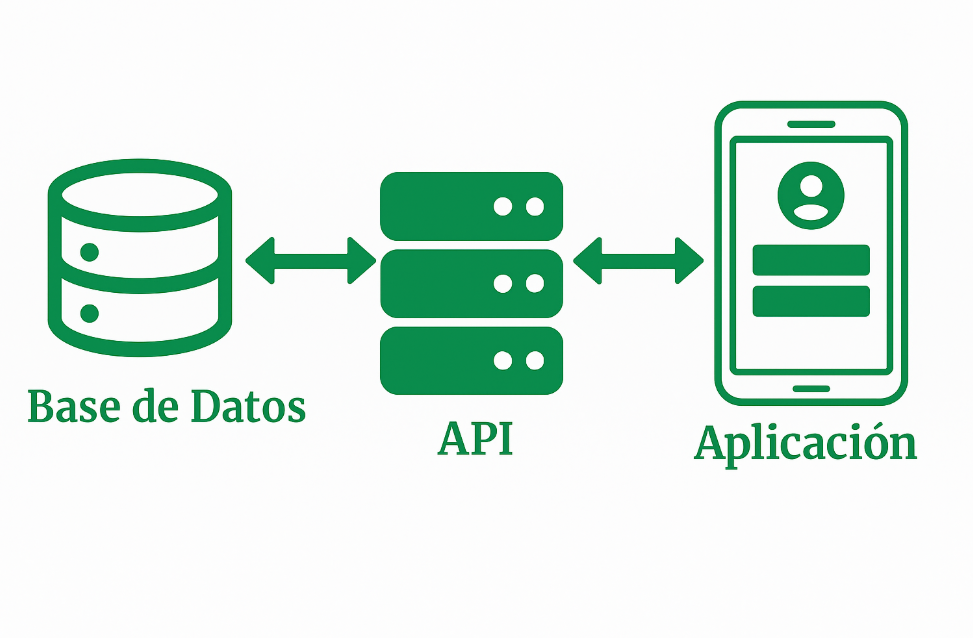
\includegraphics[width=0.8\linewidth]{Intercambio_Datos.png}
    \caption{Diseño de Datos}
    \label{D1}
\end{figure}



\section{Diseño arquitectónico}
En cuanto al diseño arquitectónico, nos referimos a la manera en que se organiza y estructura un proyecto, en este caso la aplicación GreenInHouse 2.0.

Este diseño muestra cómo el usuario interactúa con la interfaz de la aplicación, ya sea para llevar a cabo alguna acción en la que interviene también la interacción con la base de datos a través de la API, o alguna acción que no requiera de dicha comunicación con la API, como por ejemplo, cambiar el idioma de la aplicación.

Para este proyecto se ha seguido una arquitectura basada en el patrón Modelo-Vista-Controlador(MVC) extendido con una capa de servicios usada para la gestión de los datos a través de una API:
\begin{enumerate}
    \item \textbf{Modelo:}
   Se refiere a las clases de datos que se usan en la aplicación de GreenInHouse 2.0, como pueden ser:
    \begin{enumerate}
        \item {Planta}
        \item {Sensor}
        \item {Consejo}
    \end{enumerate}
    \item \textbf{Vista:}
    Se refiere a las pantallas con las que el usuario va a interactuar en la aplicación, como pueden ser:
    \begin{enumerate}
        \item {Pantalla de Gráficos}
        \item {Pantalla de Hitos}
        \item {Pantalla de Inicio}
        \item {Pantalla de Ajustes}
    \end{enumerate}
    \item \textbf{Controlador:}
    Se refiere a la lógica que hay detrás de cada acción realizada por el usuario, como puede ser:
    \begin{enumerate}
        \item {Cambio de Idioma}
        \item {Creación de Planta}
        \item {Cambio de Tierra}
    \end{enumerate}
    \item \textbf{Servicio:}
    Se refiere a todas esas llamadas HTTP (GET, POST, PUT, DELETE) que el usuario puede realizar, las cuales actúan de intermediarias entre la lógica del programa y la API.
\end{enumerate} 

Para que este diseño arquitectónico sea completamente funcional, se va a necesitar que haya conexión a internet. Dependiendo de si hay conexión a internet o no, se van a dar los siguientes casos:
\begin{enumerate}
    \item \textbf{Con Internet:}
    La mayoría de las funcionalidades de la aplicación dependen de la comunicación con la base de datos a través de la API. Para ello, se va a necesitar que tanto la maceta como el teléfono móvil estén conectados a la misma red. Estas funcionalidades incluyen:
    \begin{enumerate}
        \item {Consulta de Sensores}
        \item {Consulta de Gráficos}
        \item {Consulta de Consejos}
        \item {Crear Plantas}
        \item {Editar Plantas}
        \item {Eliminar Plantas}
    \end{enumerate}
    \item \textbf{Sin Internet:}
    Sin esta conexión a internet, la aplicación va a ser parcialmente funcional y entre estas cosas están:
    \begin{enumerate}
        \item {La interfaz carga sin problema}
        \item {Los datos guardados en el archivo ``SharedPreferences'' si que se usan.}
        \item {Funciones que no requieran de la API como el cambio de idioma}
    \end{enumerate}
\end{enumerate}


\section{Diseño procedimental}
A diferencia del diseño de arquitectura que se basaba en conocer la organización de la aplicación, el diseño procedimental se centra en ver cómo se comporta la aplicación durante su ejecución y uso. Va a mostrar la interacción entre el usuario y la aplicación y los resultados de las decisiones tomadas en tiempo de ejecución.

A continuación se verán ejemplos de diseños procedimentales de las diferentes acciones posibles dentro de la aplicación:

\subsection{Creación de una Planta:}
    \begin{enumerate}
        \item {El usuario abre la aplicación.}
        \item {Accede a la pantalla de creación de plantas.}
        \item {Rellena los campos necesarios y pulsa el botón crear planta.}
        \item {El sistema valida los campos.}
        \item {Si son válidos se envía una petición POST a la API y en caso contrario te da error y vuelves al paso 3.}
        \item {La planta se crea y queda registrada en la base de datos.}
    \end{enumerate}

\subsection{Consulta de Hitos Diarios:}
    \begin{enumerate}
        \item {El usuario abre la aplicación.}
        \item {Accede a la pantalla de hitos.}
        \item {Se hace una petición GET a la API para que devuelva tanto los datos recogidos por los sensores como los de los consejos.}
        \item {El sistema compara los datos recogidos por los sensores con los de los consejos y determina el estado del hito}
    \end{enumerate}
    
\subsection{Consulta de Gráficos:}
    \begin{enumerate}
        \item {El usuario abre la aplicación.}
        \item {Accede a la pantalla de gráficos.}
        \item {Se hace una petición GET a la API para que devuelva tanto los datos recogidos por los sensores como los de los consejos.}
        \item {El sistema compara los datos recogidos por los sensores con los de los consejos y determina el estado del gráfico}
    \end{enumerate}
    
\subsection{Consulta de Sensores:}
    \begin{enumerate}
        \item {El usuario abre la aplicación.}
        \item {Accede a la pantalla de comprobar sensores.}
        \item {Se hace una petición GET a la API para que devuelva el estado de los sensores}
    \end{enumerate}
\subsection{Modificación de una Planta:}
    \begin{enumerate}
        \item {El usuario abre la aplicación.}
        \item {Accede a la pantalla de modificar planta.}
        \item {Selecciona el tipo de planta y el nombre de la planta a modificar.}
        \item {El sistema valida los campos.}
        \item {Si son válidos se envía una petición PUT a la API y en caso contrario te da error y vuelves al paso 3.}
        \item {La planta se modifica y queda registrada en la base de datos.}
    \end{enumerate}
\subsection{Eliminación de una Planta:}
    \begin{enumerate}
        \item {El usuario abre la aplicación.}
        \item {Accede a la pantalla de eliminar planta.}
        \item {Selecciona la planta a eliminar y pulsa el botón eliminar planta.}
        \item {El sistema valida los campos.}
        \item {Si son válidos se envía una petición DELETE a la API y en caso contrario te da error y vuelves al paso 3.}
        \item {La planta se elimina de plantas activas en la base de datos y se registra como planta marchita.}
    \end{enumerate}
\apendice{Documentación técnica de programación}

\section{Introducción}
Este apéndice proporciona una guía detallada sobre la estructura del código del proyecto, las herramientas usadas para el funcionamiento de la aplicación junto con su configuración.
Se analizarán la estructrura de directorios que hay en la aplicación, además se incluirá un manual del programador en el que se explicarán cómo instalar y configurar el entorno de desarrollo junto con la ejecución del proyecto.
Con este apéndice se intenta que futuros desarrolladores que vayan a modificar o mejorar la aplicación sepan como dejar todo instalado y configurado de la mejor forma posible.

\section{Estructura de directorios}

El proyecto \textbf{GreenInHouse 2.0} sigue una estructura de directorios bien organizada, permitiendo una gestión eficiente del código, los recursos y la configuración. A continuación, se describen las principales carpetas y su contenido:

\begin{itemize}
    \item {\textbf{Directorio raíz} (\texttt{greeninhouse2/})}
    Este es el directorio principal del proyecto y contiene archivos de configuración esenciales para Flutter y Dart, además de la estructura del código fuente.

    \begin{itemize}
    \item \textbf{\texttt{.dart\_tool/}}: Carpeta generada automáticamente por Flutter y Dart con herramientas internas necesarias para la compilación.
    \item \textbf{\texttt{.idea/}}: Archivos de configuración de Android Studio para la organización del proyecto.
    \item \textbf{\texttt{build/}}: Carpeta generada durante la compilación, almacena archivos de salida del proyecto.
    \item \textbf{\texttt{ios/}, \texttt{android/}, \texttt{linux/}, \texttt{macos/}, \texttt{web/}, \texttt{windows/}}: Carpetas para cada plataforma soportada, con la configuración y código necesarios para compilar en cada sistema operativo.

    \item \texttt{\textbf{assets}/} Carpeta con todas las fotos que se van a usar en la aplicación.
    \item \textbf{\texttt{flags/}}: Carpeta con imágenes de iconos y estados de las plantas:

    \item{\texttt{\textbf{lib/}}}
    Directorio principal del código fuente en Flutter. Aquí se encuentra la lógica de la aplicación.
    \begin{itemize}
    \item \textbf{\texttt{generated/}}: Contiene archivos generados automáticamente para la internacionalización.
    \begin{itemize}
        \item \texttt{intl/l10n.dart} – Configuración de localización.
    \end{itemize}
    \item \textbf{\texttt{l10n/}}: Dedicada a la internacionalización del proyecto.
    \begin{itemize}
        \item \texttt{intl\_en.arb} – Traducciones en inglés.
        \item \texttt{intl\_es.arb} – Traducciones en español.
    \end{itemize}

    \item \textbf{\texttt{api\_service.dart}} – Implementación de las llamadas a la API.
    \item \textbf{\texttt{botones\_inicio.dart}} – Definición de la barra de navegación inferior.
    \item \textbf{\texttt{main.dart}} – Punto de entrada principal de la aplicación.

    \item \texttt{\textbf{pantalla\_graficas.dart}} – Pantalla principal con gráficos de sensores.
    \item \texttt{\textbf{pantalla\_inicio.dart}} – Pantalla inicial de la aplicación.
    \item \texttt{\textbf{pantalla\_comprobacion\_sensores.dart}} – Revisión del estado de sensores.
    \item \texttt{\textbf{pantalla\_creacionplantas.dart}} – Creación de nuevas plantas.
    \item \texttt{\textbf{pantalla\_modificarplanta.dart}} – Modificación de plantas registradas.
    \item \texttt{\textbf{pantalla\_eliminarplanta.dart}} – Eliminación de plantas registradas.

    \item \texttt{\textbf{grafica\_humedad.dart}} – Representación de datos de humedad.
    \item \texttt{\textbf{grafica\_luz.dart}} – Visualización de datos de luminosidad.
    \item \texttt{\textbf{grafica\_temperatura.dart}} – Evolución de la temperatura.
    \end{itemize}

    \item \texttt{\textbf{.gitignore}} – Define archivos y carpetas a excluir del repositorio Git.
    \item \texttt{.metadata} – Archivo interno de configuración de Flutter.
    \item \texttt{\textbf{analysis\_options.yaml}} – Reglas de análisis de código en Dart.
    \item \texttt{\textbf{greeninhouse2.iml}} – Configuración de IntelliJ/Android Studio.
    \item \texttt{\textbf{pubspec.yaml}} – Define dependencias, assets e información del proyecto.
    \item \texttt{\textbf{pubspec.lock}} – Registro de versiones de las dependencias utilizadas.
    \item \texttt{\textbf{README.md}} – Documentación inicial sobre el proyecto y su instalación.
    \end{itemize}
\end{itemize}

\section{Manual del programador}
El objetivo del manual del programador es la de proporcionar una guía del desarrollo y mantenimiento de la aplicación. Este manual está dirigido a desarrolladores que necesiten como funciona las herramientas utilizadas en el desarrollo de esta aplicación.
También se ha incluido las instrucciones necesarias para configurar el entorno de desarrollo y ejecutar la aplicación.
Además, se ha detallado aspectos que son claves como la estructura de datos que sigue la aplicación y la comunicación con la API entre otras cosas con el objetivo de facilitar mejoras que se puedan llevar a cabo en un futuro.


\subsection{\textbf{Instalación de Android Studio}}
Android Studio es el entorno de desarrollo integrado (IDE) oficial que se usa en el desarrollo de apps para Android. Basado en el potente editor de código y las herramientas para desarrolladores de IntelliJ IDEA.
Se puede descargar desde su página oficial: \url{https://developer.android.com/studio?hl=es-419}



Al descargar la aplicación y ejecutarla nos saldrá lo que vemos en la foto a continuación y le daremos al botón de ``Next''.\ref{C1}
\begin{figure}[H]
    \centering
    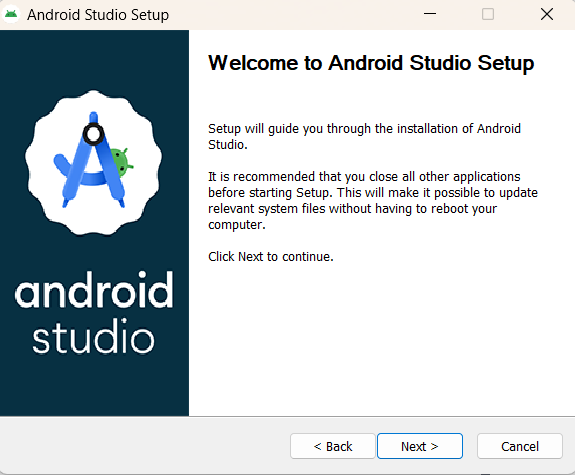
\includegraphics[width=0.8\linewidth]{AndroidStudio1.png}
    \caption{Le daremos a Next.}
    \label{C1}
\end{figure}

Tras esto nos saldrá la siguiente ventana en la que dejaremos lo que viene por defecto y le volveremos a dar a ``Next''.\ref{C2}
\begin{figure}[H]
    \centering
    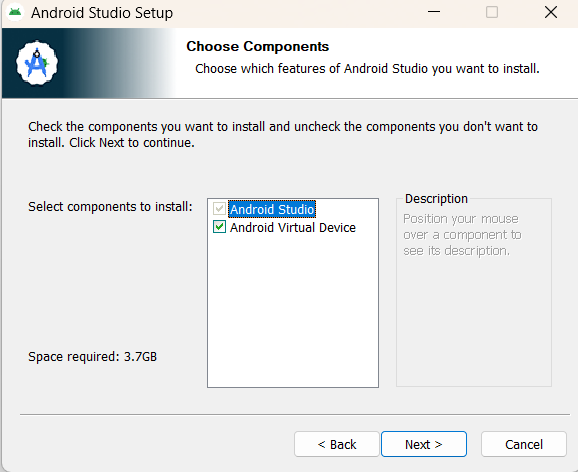
\includegraphics[width=0.8\linewidth]{AndroidStudio2.png}
    \caption{Volvemos a darle a Next}
    \label{C2}
\end{figure}

Por último en la ultima ventana decidiremos el path donde instalar la aplicación y le daremos a ``Next'' para que instale la aplicación en el path seleccionado.\ref{C3}
\begin{figure}[H]
    \centering
    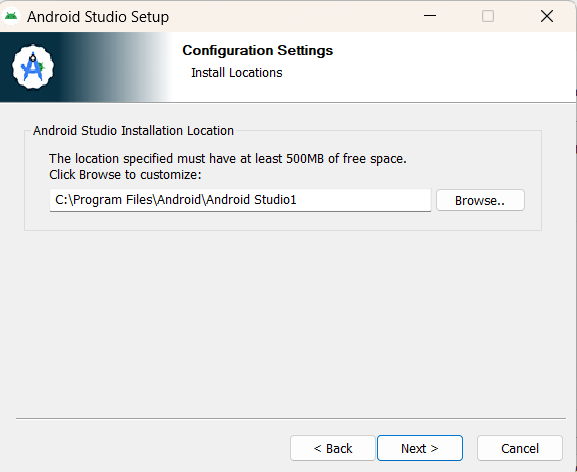
\includegraphics[width=0.8\linewidth]{AndroidStudio3.png}
    \caption{Elegir path y darle a Next}
    \label{C3}
\end{figure}

Tras instalar Android Studio vamos a pasar a la configuración de las herramientas instalando tanto Flutter como Dart.
Esto se hace entrando en la pestaña de ajustes y en Plugins.\ref{C4}

\begin{figure}[H]
    \centering
    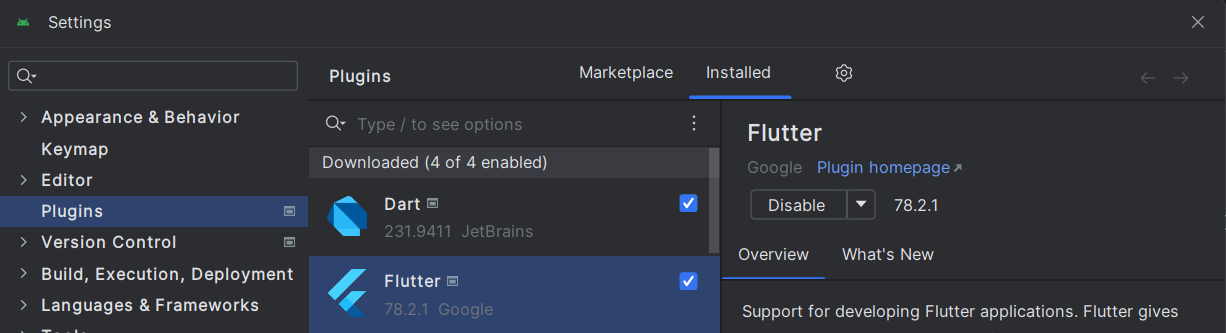
\includegraphics[width=0.8\linewidth]{PlugingsAndroidStudio.png}
    \caption{Instalación plugins Android Studio}
    \label{C4}
\end{figure}


El siguiente paso es la configuración de SDK en el Android Studio. Esto se hace accediendo a ajustes y alli desde Languages \& Frameworks. \ref{C5}

\begin{figure}[H]
    \centering
    \includegraphics[width=0.8\linewidth]{Configuración-SDK-AndroidStudio.png}
    \caption{Configuración de SDK en Android Studio}
    \label{C5}
\end{figure}


Por ultimo vamos a instalar unas herramientas en SDK Tools que viene a la derecha de la de SDK Platforms necesarias para el buen funcionamiento de la herramienta.\ref{C6}

\begin{figure}[H]
    \centering
    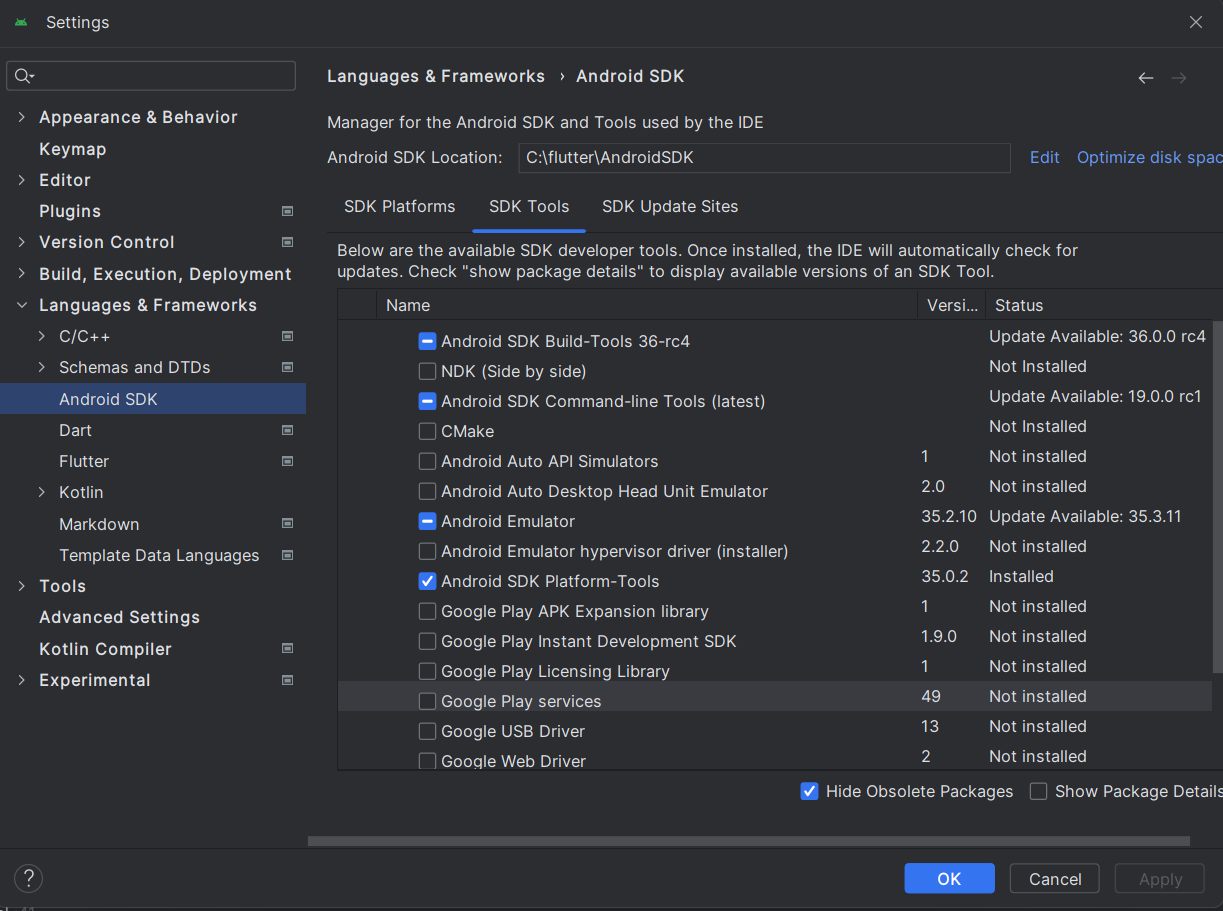
\includegraphics[width=0.8\linewidth]{Configuracion-SDKTools-AndroidStudio.png}
    \caption{Instalación de Herramientas de SDK}
    \label{C6}
\end{figure}

\subsection{\textbf{Instalación de Flutter}}
Para la instalación de Flutter deberemos ir a su página web y descargarlo. Alli nos preguntarán por nuestro sistema operativo, tras elegirlo nos preguntarán por el tipo de aplicación queremos ya sea ``Android'' o ``Web'' o ``Desktop''. En mi caso, seleccioné ``Windows'' y ``Android''. Tras esto nos descargaremos el .zip que aparece en la web como se puede ver en la imagen a continuación.

\begin{figure}[H]
    \centering
    \includegraphics[width=0.8\linewidth]{Instalación_Flutter_SDK.png}
    \caption{Descargaremos el archivo}
    \label{C7}
\end{figure}

A continuación, deberemos descomprimir el .zip y guardar la carpeta en un directorio que elijamos para de esta manera poder añadir en las variables de entorno la ruta del fichero ``\textbackslash bin''.

Primero, abriremos la configuración avanzada del sistema desde el buscador de Windows y nos saldrá la pantalla que vemos en la siguiente captura. Daremos al botón que pone ``Variables de entorno'' para continuar.

\begin{figure}[H]
    \centering
    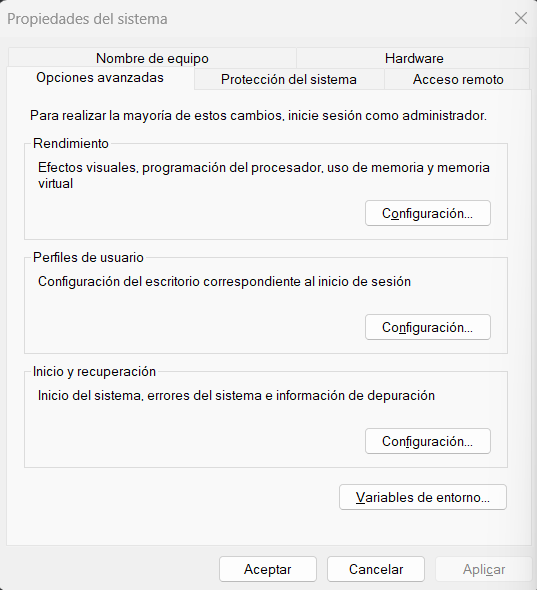
\includegraphics[width=0.8\linewidth]{Variables_Entorno_1.png}
    \caption{Le daremos al botón de ``Variables de entorno''}
    \label{C8}
\end{figure}

Seguido, buscaremos la variable que se llame ``Path'' y le daremos al botón de ``Editar'' como vemos en la captura siguiente.

\begin{figure}[H]
    \centering
    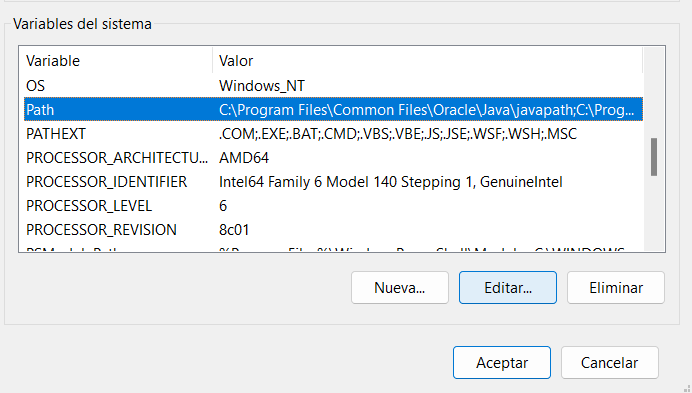
\includegraphics[width=0.8\linewidth]{Variables_Entorno_2.png}
    \caption{Seleccionaremos la variable ``Path'' y le daremos a ``Editar''}
    \label{C9}
\end{figure}

Por último, le daremos al botón de ``Nuevo'' y añadiremos la ruta donde se encuentre nuestra carpeta ``\textbackslash bin''. Nos quedará añadido como se puede ver en la siguiente imagen y le daremos a ``Aceptar'' para que se quede guardado.

\begin{figure}[H]
    \centering
    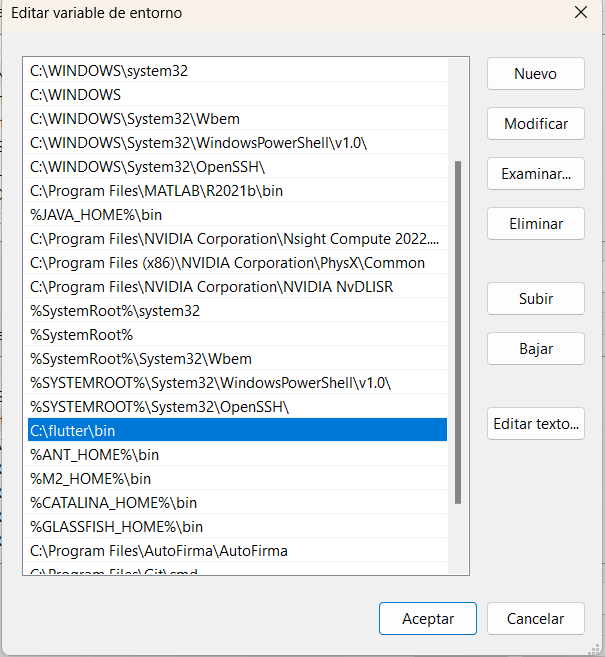
\includegraphics[width=0.8\linewidth]{Variables_Entorno_3.png}
    \caption{Añadiremos el \textit{path} de ``\textbackslash bin'' y le daremos a ``Aceptar''}
    \label{C10}
\end{figure}

Para comprobar que todo se ha instalado correctamente abriremos una terminal y mediante el comando \textit{``flutter doctor''} verificaremos que se ha instalado bien y si falta alguna configuración o dependencia.

\begin{figure}[H]
    \centering
    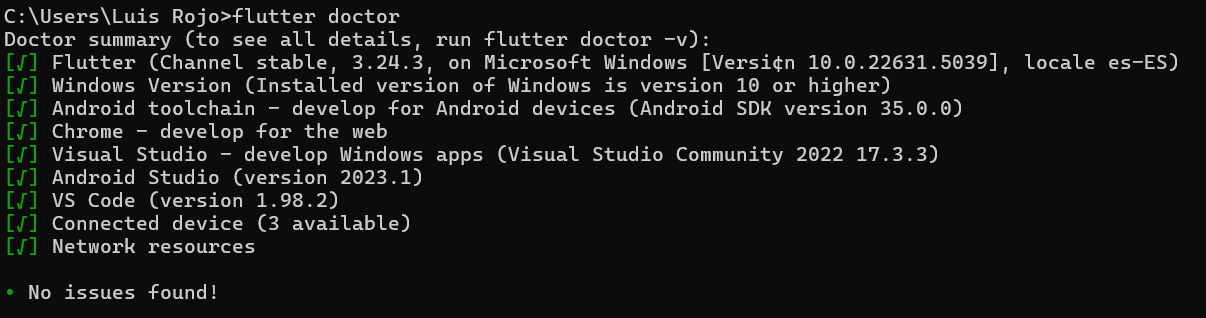
\includegraphics[width=0.8\linewidth]{Comando_flutterdoctor.png}
    \caption{Uso del comando \textit{''flutter doctor''}}
    \label{C11}
\end{figure}

\section{Compilación, instalación y ejecución del proyecto}

Para poder probar y utilizar la aplicación de GreenInHouse 2.0 durante su desarrollo ha sido necesario el uso de un emulador. El propio AndroidStudio tiene sus propios emuladores los cuales puedes descargar y configurar en función de tus intereses de la aplicación.

Para poder llevar a cabo la ejecución del programa primero deberemos descargarnos el proyecto mediante el uso del comando:
\begin{verbatim}
git clone https://github.com/LuisRojoSanz/GreenInHouse2_APP
\end{verbatim}

Tras esto se habrá descargado el contenido del repositorio de github y se podrá ejecutar el proyecto.

Primero se deberá pulsar el botón del ``+'' en \textit{Device Manager} para empezar a descargar el emulador como se ve en la imagen a continuación.

\begin{figure}[H]
    \centering
    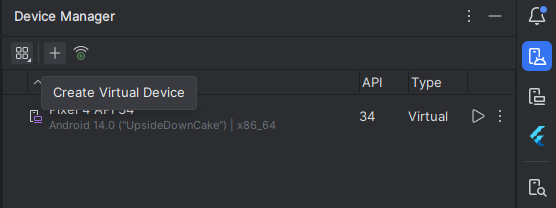
\includegraphics[width=0.8\linewidth]{InstalacionyEjecucion1.png}
    \caption{Descarga de un emulador}
    \label{C12}
\end{figure}

Una vez se haya pulsado el ``+'' saldrá la captura a continuación en la que se seleccionará el modelo de emulador deseado y se dara a ``Next''.

\begin{figure}[H]
    \centering
    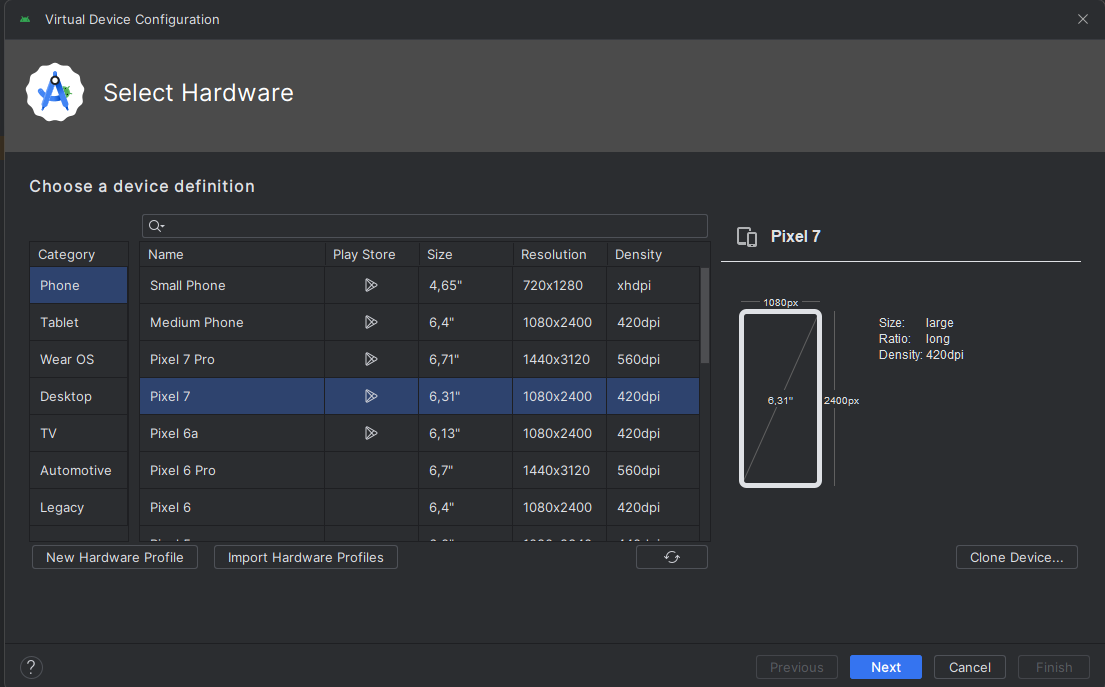
\includegraphics[width=0.8\linewidth]{InstalacionyEjecucion2.png}
    \caption{Seleccionando un emulador}
    \label{C13}
\end{figure}

Tras esto habrá que seleccionar la versión de Android que mejor funcione para el proyecto y darle al botón de ``Next''

\begin{figure}[H]
    \centering
    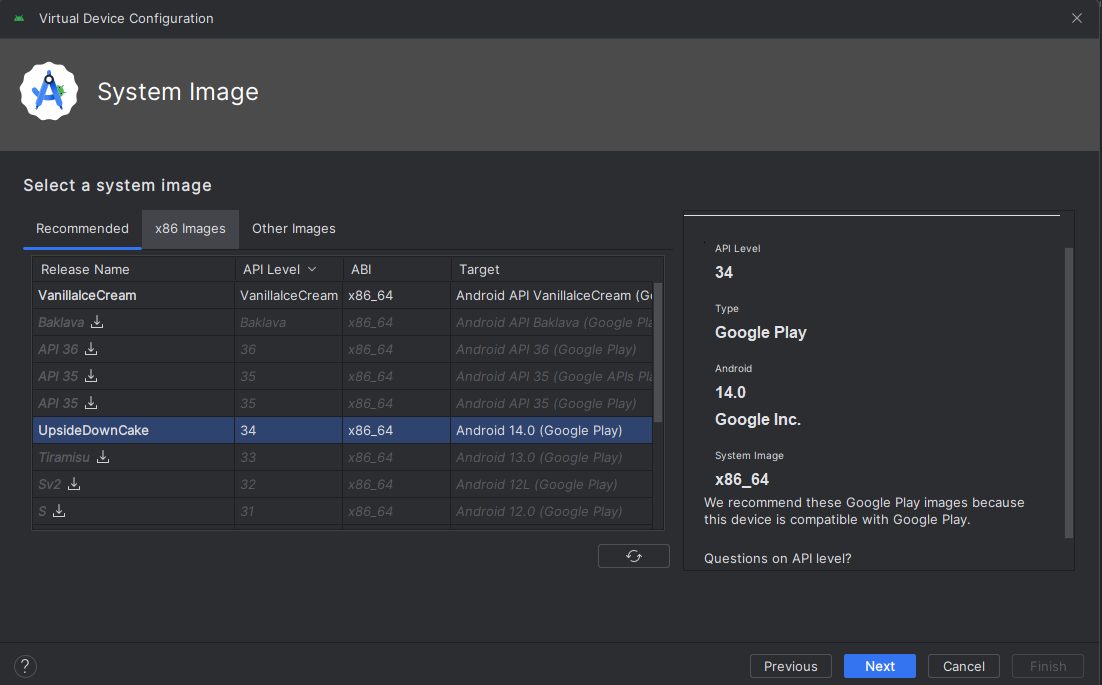
\includegraphics[width=0.8\linewidth]{InstalacionyEjecucion3.png}
    \caption{Seleccionando la versión de Android del emulador}
    \label{C14}
\end{figure}

En la siguiente pantalla se deberá verificar la configuración del emulador y seleccionar el nombre que de desee. Una vez verificado se dará al botón de ``Next''.

\begin{figure}[H]
    \centering
    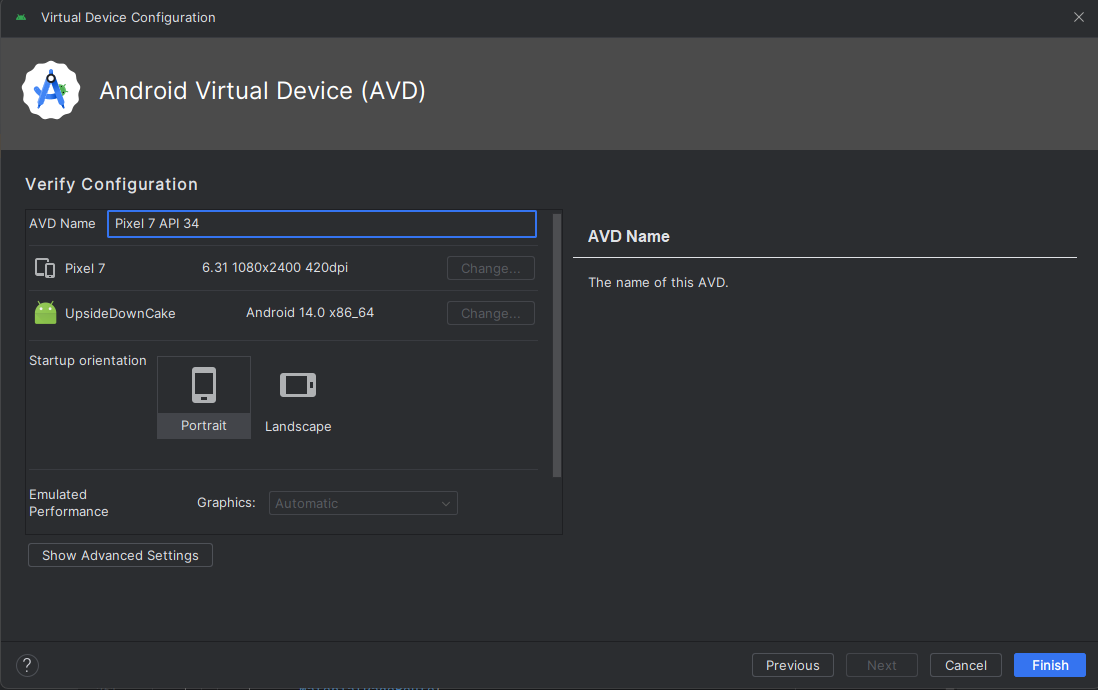
\includegraphics[width=0.8\linewidth]{InstalacionyEjecucion4.png}
    \caption{Verificar la configuración del emulador}
    \label{C15}
\end{figure}

Descargado ya el emulador ahora tocará seleccionarlo como vemos en la imagen a continuación del emulador que esta resaltado en azul. Una vez seleccionado, se empezará a ejecutar el emulador.

\begin{figure}[H]
    \centering
    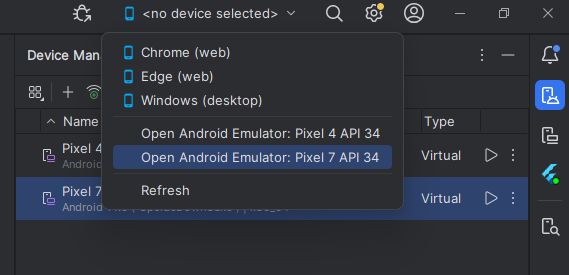
\includegraphics[width=0.8\linewidth]{InstalacionyEjecucion5.png}
    \caption{Ejecución del emulador}
    \label{C16}
\end{figure}

Por último, una vez que el emulador ya ha iniciado como vemos en la siguiente imagen, se deberá pulsar el botón verde de ejecutar de arriba a la izquierda que está rodeado en azul. Una vez pulsemos este botón se comenzará a ejecutar el proyecto.

\begin{figure}[H]
    \centering
    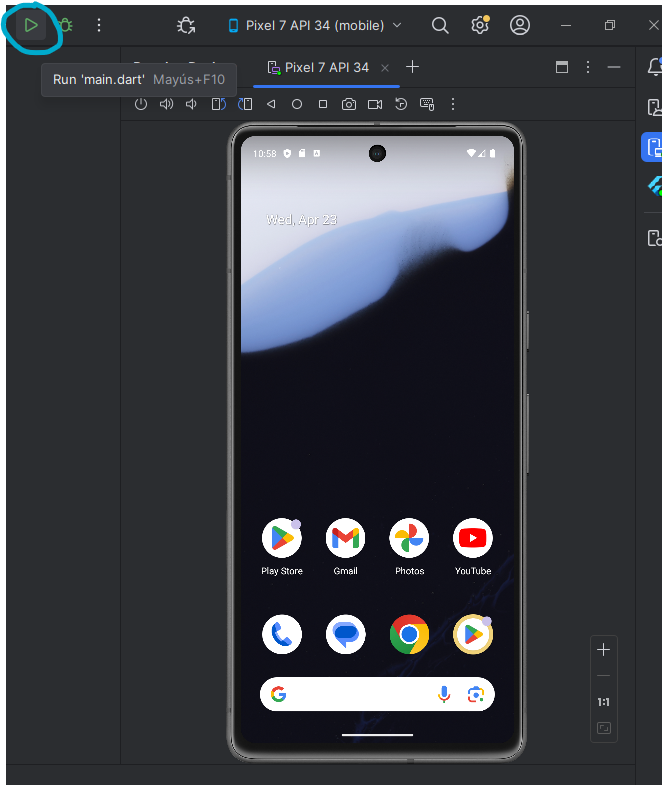
\includegraphics[width=0.8\linewidth]{InstalacionyEjecucion6.png}
    \caption{Ejecución del proyecto}
    \label{C17}
\end{figure}


\section{Pruebas del sistema}
Para garantizar que la aplicación GreenInHouse 2.0 funciona de manera correcta se han llevado a cabo diferentes tipos de pruebas: 

\subsection{Pruebas Funcionales:} Estas pruebas se basan en comprobar que cada uno de las funcionalidades de los requisitos funciona de manera correcto como por ejemplo:
    \begin{enumerate}
        \item \textbf{Crear Planta:} El sistema permite que el usuario pueda seleccionar el nombre y tipo de planta y crear la planta.
        \item \textbf{Consultar Hitos}: La comunicación con la base de datos a través de la API hace que se puedan ver los hitos diarios.
        \item \textbf{Cambiar Idioma:} El usuario selecciona el idioma que desee y automaticamente se cambio el idioma en toda la aplicación.
        \item \textbf{Seleccionar Imagen de Planta:} El usuario puede sacar una foto con la cámara o seleccionarla de la galería.
    \end{enumerate}
\subsection{Pruebas de Integración:} Estas pruebas se realizan comprobando la comunicación entre la aplicación y la base de datos mediante diferentes peticiones HTTP dentro de la red local. Estas peticiones pueden ser:
    \begin{enumerate}
        \item \textbf{GET}
        \item \textbf{POST}
        \item \textbf{PUT}
        \item \textbf{DELETE}
    \end{enumerate}
\subsection{Pruebas de Interfaz de Usuario:} Este tipo de pruebas tienen que ver con el correcto funcionamiento lo visible para el usuario como puede ser:
    \begin{enumerate}
        \item \textbf{Funcionamiento de botones y demás \textit{widgets}:} Se han hecho pruebas para comprobar que tanto los botones como los demás elementos con los que puede interactuar el usuario de la interfaz funcionen de manera correcta.
        \item \textbf{Adaptabilidad:} Se han hecho pruebas para comprobar que usando telefónos móviles de diferentes resoluciones la interfaz se adapta de manera correcta.
    \end{enumerate}
\subsection{Pruebas Simulando Fallos:}
Se han hecho también pruebas simulando fallos para ver como reaccionaba la aplicación. Este tipo de pruebas han sido por ejemplo:
    \begin{enumerate}
        \item \textbf{Sin Conexion a Internet:} Se han hecho pruebas pruebas para ver como reaccionaba la aplicación en caso de que no hubiera conexión a internet y por tanto no se pudiera comunicar la aplicación con la API. Se ha observado que la aplicación sigue funcionando solo que no ofrece dichos servicios que necesitan de los datos de la base de datos.
        \item \textbf{Plantas con el mismo nombre:} Se han hecho pruebas intentando crear una planta con el mismo nombre que otra ya existente. Al intentar esta prueba la aplicación ha dado error debido a la existencia de una planta con ese mismo nombre.
    \end{enumerate}
    
\apendice{Documentación de usuario}

\section{Introducción}

\section{Requisitos de usuarios}

\section{Instalación}

\section{Manual del usuario}



\apendice{Anexo de sostenibilización curricular}

\section{Introducción}
Este anexo incluirá una reflexión personal del alumnado sobre los aspectos de la sostenibilidad que se abordan en el trabajo.
Se pueden incluir tantas subsecciones como sean necesarias con la intención de explicar las competencias de sostenibilidad adquiridas durante el alumnado y aplicadas al Trabajo de Fin de Grado.

Más información en el documento de la CRUE \url{https://www.crue.org/wp-content/uploads/2020/02/Directrices_Sosteniblidad_Crue2012.pdf}.

Este anexo tendrá una extensión comprendida entre 600 y 800 palabras.



\bibliographystyle{plain}
\bibliography{bibliografiaAnexos}

\end{document}
